\documentclass{article}
\usepackage{amsmath, amssymb, amsfonts}
\usepackage{fullpage}
\usepackage{enumerate}
\usepackage{graphicx}

\title{CS 4780/5780 Homework 9\vspace{-10pt}}
\author{Due: Tuesday 12/11/18 11:55pm on Gradescope}
\date{}

\begin{document}
    \maketitle
    \section*{Problem 1: Neural Nets and kernel machines.}
    Assume you are given a 1-hidden layer neural network, with $M$ hidden nodes. Let $\vec{x}$ denote the input, the hidden nodes $h_{m}(\vec{x})$ (for $m=1,\dots,M$) and the output $H(\vec{x})$
    We could view a one-hidden-layer neural network as kernelized linear regression with a learned kernel. What is the kernel function?
     \section*{Problem 2: Convolutional Process}
     \begin{enumerate}
     	\item Suppose you have a filter of size $k \times k$ and stride s. When you apply this filter to a $n \times n$ input with padding $p$, what is the dimension of the output feature map? 
     	\item Suppose you are given an $3 \times 3$ matrix from one patch of an image $I$ and a $3\times 3$ convolutional kernel $K$. In the image matrix, each entry represents the gray scale color of a corresponding pixel.
     	$$I = \begin{bmatrix}
     	3 & 1&  1 \\
     	3 & 0 & 2 \\
     	4 & 4 & 0
     	\end{bmatrix}$$ and $$K = \begin{bmatrix}
     	1 & 0 \\ 0 & 1   
     	\end{bmatrix}$$
     	What is the output of applying the filter to the input with stride 1 without padding?
     \end{enumerate}
    \newpage
    \section*{Problem 3: RELU-network}
    In this question, you are going to explore a 2-layer
    fully connected network with RELU activation function. 
    \begin{figure}[h!]
        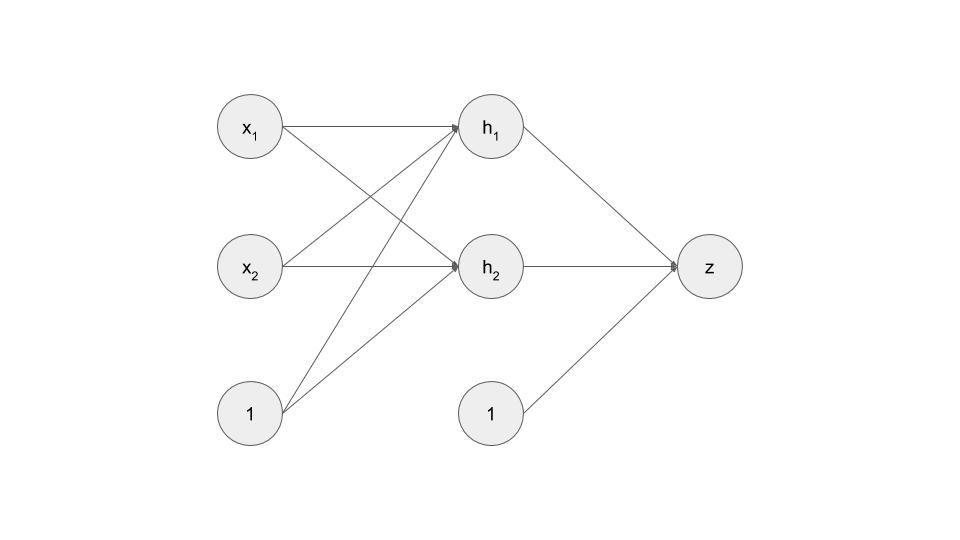
\includegraphics[width=\textwidth]{nn.jpg}
    \end{figure}
    \newline
    Suppose you have the architecture above, namely, 
    \begin{align*}
        \begin{bmatrix}h_1 \\ h_2 \end{bmatrix} &= \begin{bmatrix}w_{11} & w_{12} & w_{13} \\w_{21} & w_{22} & w_{23}\end{bmatrix} \begin{bmatrix} x_1 \\ x_2 \\ 1\end{bmatrix} \\
        z &= \begin{bmatrix} v_1 & v_2 & v_3\end{bmatrix} \begin{bmatrix}
        f(h_1) \\ f(h_2) \\ 1 
        \end{bmatrix}  \\
        t &= \sigma(z) 
    \end{align*}
    where $f(h_i) = max(0, h_i)$, $\sigma(z) = \frac{1}{1 + e^{-z}}$ and $t$ is the output of the network.

    \begin{enumerate}[(a)]
        \item Suppose $\begin{bmatrix}w_{11} & w_{12} & w_{13} \\w_{21} & w_{22} & w_{23}\end{bmatrix} = \begin{bmatrix}1 & -1 & 0 \\-1 & -1 & 0\end{bmatrix}$ and $\begin{bmatrix} v_1 & v_2 & v_3\end{bmatrix} = \begin{bmatrix} 1 & 1 & -2\end{bmatrix}$. Draw the decision boundary of the network, namely, $\sigma(z) = 0.5$ within the range $[-10, 10] \times [-10, 10]$. Please indicate the positive and negative side of the boundary. 
        \item Assume the weights in (a), what is the prediction for $[x_1, x_2]^T = [1,1]^T$?
        \item Usually, the weights $W = \begin{bmatrix}w_{11} & w_{12} & w_{13} \\w_{11} & w_{12} & w_{13}\end{bmatrix}$ and $V = \begin{bmatrix} v_1 & v_2 & v_3\end{bmatrix}$have to be learned using Stochastic Gradient Descent. For neural network binary classification, a common loss function is the cross entropy loss
        $$l(y, t) = - (y \log (t) + (1 -y) \log (1-t))$$ where $y$ is the true label for a sample and $t$ is the output of the neural network. In order to use SGD, we have to derive the gradient with respect to $W$ and $V$. Show that for a single training example, $x = [x_1, x_2]$
        \begin{align*}
            \frac{\partial l}{\partial v_i} &= (t - y) f(h_i) \text{ for } i \neq 3 \\
            \frac{\partial l}{\partial v_3} &= (t - y) \\
            \frac{\partial l}{\partial w_{ij}} &= (t - y) v_i \mathbb{I}(h_i > 0) x_j \text{ for } j \neq 3\\
            \frac{\partial l}{\partial w_{i3}} &= (t - y) v_i \mathbb{I}(h_i > 0) 
        \end{align*}
        where $\mathbb{I}(\cdot)$ is the indicator function. 
    \end{enumerate}
\end{document}